% Author: Till Tantau
% Source: The PGF/TikZ manual
\documentclass{standalone}

\usepackage{tikz}
\usetikzlibrary{mindmap,trees}
\usepackage{verbatim}

\begin{document}
\pagestyle{empty}

\begin{comment}
:Title: Computer science mindmap
:Tags: Manual, Mindmap

Version 1.09 of PGF/TikZ added a library for drawing mindmaps. Here's an example
from the manual. 

| Author: Till Tantau
| Source: The PGF/TikZ manual
3
\end{comment}

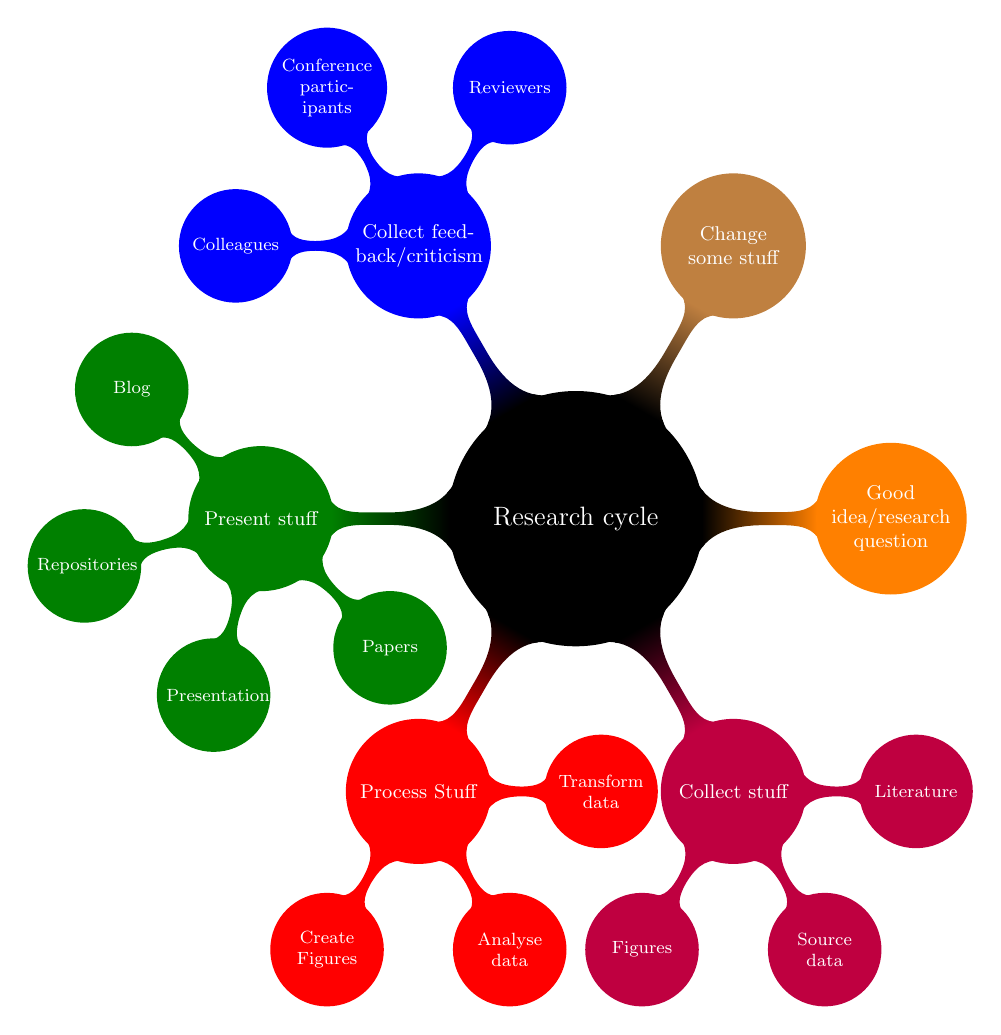
\begin{tikzpicture}[node distance = 2cm, auto, scale=0.8, transform shape]
  \path[mindmap,concept color=black,text=white]
      node[concept] {Research cycle}
    [clockwise from=0]
    child[concept color=orange] { node[concept] {Good idea/research question} }
    child[concept color=purple] { 
	node[concept] {Collect stuff} 
      [clockwise from=0]
      child { node[concept] {Literature} }
      child { node[concept] {Source data} }
      child { node[concept] {Figures} }
    } 
    child[concept color=red] { node[concept] {Process Stuff} 
      [clockwise from=0]
      child { node[concept] {Transform data} }
      child { node[concept] {Analyse data} }
      child { node[concept] {Create Figures} }
	}
    child[concept color=green!50!black] {
      node[concept] {Present stuff}
      [clockwise from=315]
      child { node[concept] {Papers} }
      child { node[concept] {Presentation} }
      child { node[concept] {Repositories} }
      child { node[concept] {Blog} }
    }  
    child[concept color=blue] {
      node[concept] {Collect feedback/criticism}
      [clockwise from=180]
      child { node[concept] {Colleagues} }
      child { node[concept] {Conference participants} }
      child { node[concept] {Reviewers} }
    }
    child[concept color=brown] { node[concept] {Change some stuff} };
\end{tikzpicture}
\end{document}